% Chapter 3

\chapter{Algorithms, Source Code, the Portable Graphics Format and Acronyms} % Main chapter title
\label{chap:Chapter3} % For referencing the chapter elsewhere, use \ref{chap:Chapter3} 

%----------------------------------------------------------------------------------------
\section{Algorithms}

 \LaTeX{}  has several packages for typesetting algorithms in form of ''pseudocode''. In this template, we suggest the use of the \verb|algorithm| environment with the \verb|algpseudocode| package. 
More information about algorithms can be found at \url{https://en.wikibooks.org/wiki/LaTeX/Algorithms}.

Algorithm~\ref{alg:euclid} shows Euclid's algorithm that computes  Greatest Common Divisor (GCD) of two integer numbers.

\begin{algorithm}[b]
\caption{Euclid’s algorithm}
\label{alg:euclid}
\begin{algorithmic}[1]
\scriptsize

\State \textbf{Input}: Two integer numbers, $a$ and $b$
\State \textbf{Output}: GCD of $a$ and $b$
\State
\Procedure{Euclid}{$a,b$}\Comment{The GCD of $a$ and $b$}
\State $r\gets a\bmod b$
\While{$r\not=0$}\Comment{We have the answer if $r$ is $0$}
\State $a\gets b$
\State $b\gets r$
\State $r\gets a\bmod b$
\EndWhile
\State \textbf{return} $b$\Comment{The GCD is $b$}
\EndProcedure

\end{algorithmic}
\end{algorithm}

Here it is the \LaTeX{} text for the ''pseudocode'' algorithm presented in  Algorithm~\ref{alg:euclid}.

\begin{verbatim}
\begin{algorithm}
\caption{Euclid’s algorithm (pseudocode)}
\label{alg:euclid}
\begin{algorithmic}[1]
\scriptsize

\State \textbf{Input}: Two integer numbers, $a$ and $b$
\State \textbf{Output}:  Greatest Common Divisor (GCD) of $a$ and $b$
\State
\Procedure{euclid}{$a,b$}\Comment{The GCD of $a$ and $b$}
\State $r\gets a\bmod b$
\While{$r\not=0$}\Comment{We have the answer if $r$ is $0$}
\State $a\gets b$
\State $b\gets r$
\State $r\gets a\bmod b$
\EndWhile
\State \textbf{return} $b$\Comment{The GCD is $b$}
\EndProcedure

\end{algorithmic}
\end{algorithm}
\end{verbatim}

\verb|\listofalgorithms| command generates a list of all algorithms. This command is called in the \file{frontmatter.tex} file. Therefore, if there is no algorithm in the thesis, this command must be removed (or commented) from such file.

\section{Source Code}
Sometimes there is the need to present programming source code snippets.
The \verb|listings| package  is a powerful way to get nice source code highlighting in \LaTeX{}. It supports various programming languages, like Java (selected as the default language in this template), C, and many others.

Listing~\ref{lst:euclid_java} and Listing~\ref{lst:euclid_c} show the source code of the Euclid’s algorithm, written in Java and C, respectively.

\begin{minipage}{\linewidth}
\lstinputlisting [language=Java,
	caption=Euclid’s algorithm (Java).,
	label=lst:euclid_java]
{ch3/assets/euclid.java}
\end{minipage}

\begin{minipage}{\linewidth}
\lstinputlisting [language=C, 
	caption=Euclid’s algorithm (C).,
	label=lst:euclid_c,
	numbers=none]
{ch3/assets/euclid.c}
\end{minipage}

Here it is the \LaTeX{} text for both listings. Note that we encapsulate the listings inside a \verb|\minipage| so that the listing does note break across pages.
Using the \verb|\lstinputlisting| command, the source code must be written in a separate file. In these two cases, both files are in \path{ch3\assets\} directory.

\begin{verbatim}
\begin{minipage}{\linewidth}
\lstinputlisting [language=Java,
    caption=Euclid’s algorithm (Java).,
    label=lst:euclid_java]
{ch3/assets/euclid.java}
\end{minipage}

\begin{minipage}{\linewidth}
\lstinputlisting [language=C, 
    caption=Euclid’s algorithm (C).,
    label=lst:euclid_c,
    numbers=none]
{ch3/assets/euclid.c}
\end{minipage}

\end{verbatim}
As it can be seen from the text above, there are a lot of parameters that can be specified, like programming language (\verb|language|), numbering, etc.   
More information about listings can be found at 
\url{https://en.wikibooks.org/wiki/LaTeX/Source_Code_Listings} and 
\url{http://texdoc.net/texmf-dist/doc/latex/listings/listings.pdf}.


\verb|\listoflisting| command generates a list of all source code listings. This command is called in the \file{frontmatter.tex} file. Therefore, if there are no listings in the thesis, this command must be removed (or commented) from such file.

\section{The Portable Graphics Format}
The \gls{PGF} and a number of packages built on top of \gls{PGF} (such as TiKZ and PGFPLOTS) enable producing high quality graphical elements for your document. 
 
\subsection{TiKZ}
TikZ is built on top of PGF and allows you to create sophisticated graphics using \LaTeX{} commands. According to its author, Till Tantau~\footnote{Available online at \url{ftp://ftp.di.uminho.pt/pub/ctan/graphics/pgf/base/doc/pgfmanual.pdf}},  "\textit{What is TikZ? Basically, it just defines a number of \TeX{} commands
that draw graphics.}". With TikZ it is possible to accurately position picture elements, use \LaTeX{} fonts, incorporate mathematical typesetting, and use other \LaTeX{} features in your drawings.

The TikZ package defines the \verb|tikzpicture| environment that is required to draw a graphic. 
This environment must be inserted into a \verb|figure| environment when numbering and caption are required.
Figure~\ref{fig:tikz} shows a simple use of TiKZ, for which the \LaTeX{} source is as follows.

\begin{verbatim}
\begin{figure}[t]
\centering


\begin{tikzpicture}
% Define four points
\coordinate (P0) at (1,0);
\coordinate (P1) at (0,1);
\coordinate (P2) at (-1,0);
\coordinate (P3) at (0,-1);
% Draw the diamond
\draw (P0)--(P1)--(P2)--(P3)--cycle;
\end{tikzpicture}

\caption{Using TiKZ for drawing pictures.}
\label{fig:tikz}
\end{figure}
\end{verbatim}

\begin{figure}[h]
\centering


\begin{tikzpicture}
% Define four points
\coordinate (P0) at (0,0);
\coordinate (P1) at (1,0);
\coordinate (P2) at (0,1);
\coordinate (P3) at (-1,0);
\coordinate (P4) at (0,-1);
% Draw the diamond
\draw (P1)--(P2)--(P3)--(P4)--cycle;
\end{tikzpicture}

\caption{Using TiKZ for drawing pictures.}
\label{fig:tikz}
\end{figure}


A great amount of examples are available at \url{http://www.texample.net/tikz/examples/}. 
More information about TiKZ can be found at 
\url{https://en.wikibooks.org/wiki/LaTeX/PGF/TikZ} and 
\url{ftp://ftp.di.uminho.pt/pub/ctan/graphics/pgf/base/doc/pgfmanual.pdf}.

\subsection{PGFPLOTS}

PGFPLOTS provides tools to draw high quality plots, and is based on TiKZ. To use PGFPLOTS in the thesis you need to use \verb|\usepackage{pgfplots}| (in \file{main.tex}).
To guarantee compatibility you need to specify \verb|\pgfplotsset{compat=<version>}|.
You can choose the \verb|version| ().
In this case, it is recommended to choose \verb|newest|. The choice \verb|compat=newest| means "I do not care if my old figures change in appearance after the next version upgrade".

Here it is the \LaTeX{} text for create the graph presented in Figure~\ref{fig:pgfplots}.
\begin{verbatim}
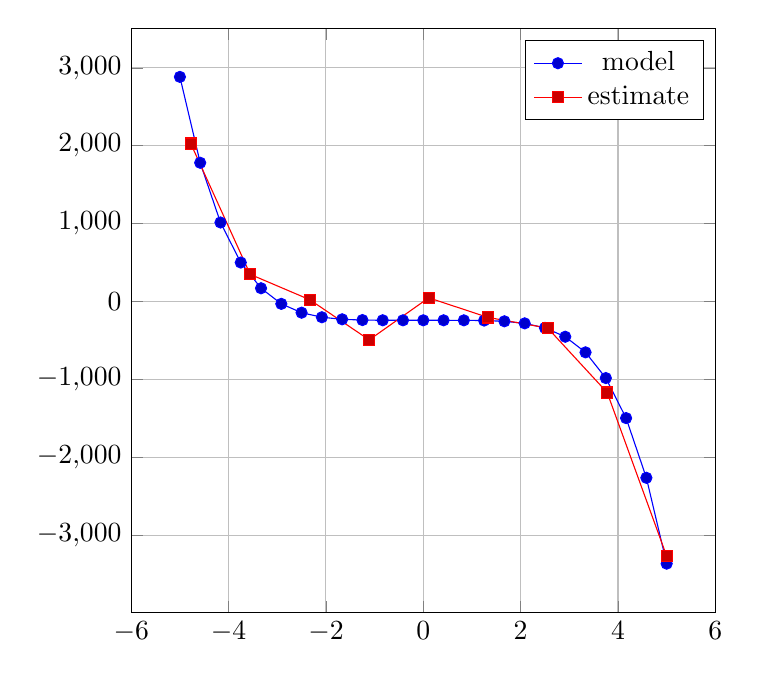
\begin{tikzpicture} 
	\begin{axis}[ height=9cm, width=9cm, grid=major, ] 
		\addplot {-x^5 - 242}; 
		\addlegendentry{model}
		\addplot coordinates { 
			(-4.77778,2027.60977) 
			(-3.55556,347.84069) 
			(-2.33333,22.58953) 
			(-1.11111,-493.50066) 
			(0.11111,46.66082) 
			(1.33333,-205.56286) 
			(2.55556,-341.40638) 
			(3.77778,-1169.24780) 
			(5.00000,-3269.56775) 
		}; 
		\addlegendentry{estimate} 
	\end{axis} 
\end{tikzpicture}
\end{verbatim}

Figure~\ref{fig:pgfplots} shows an example of a graph created using PGFPLOTS functions.

\begin{figure}[h]
\centering
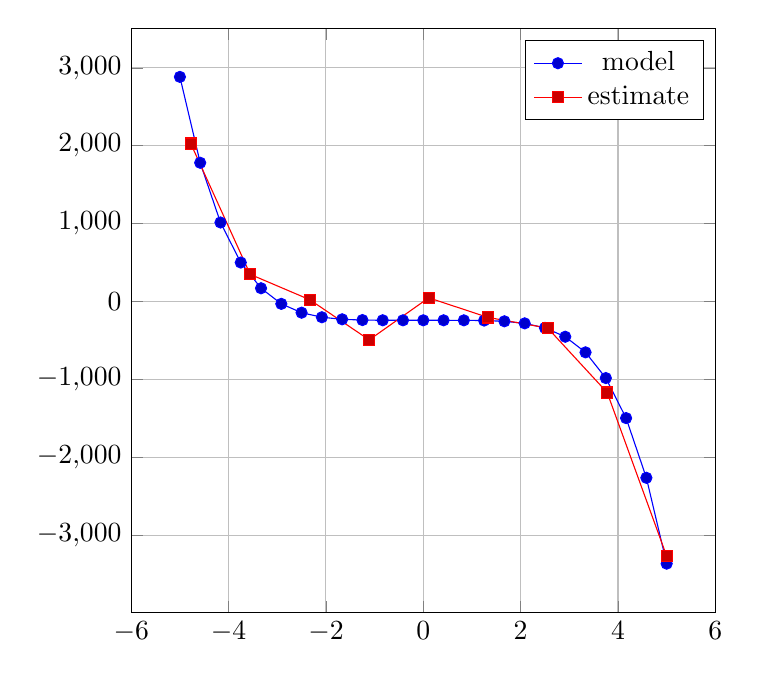
\begin{tikzpicture} 
	\begin{axis}[ height=9cm, width=9cm, grid=major, ] 
		\addplot {-x^5 - 242}; 
		\addlegendentry{model}
		\addplot coordinates { 
			(-4.77778,2027.60977) 
			(-3.55556,347.84069) 
			(-2.33333,22.58953) 
			(-1.11111,-493.50066) 
			(0.11111,46.66082) 
			(1.33333,-205.56286) 
			(2.55556,-341.40638) 
			(3.77778,-1169.24780) 
			(5.00000,-3269.56775) 
		}; 
		\addlegendentry{estimate} 
	\end{axis} 
\end{tikzpicture}
\caption{Using PGFPLOTS for drawing a graph.}
\label{fig:pgfplots}
\end{figure}

A great amount of examples are available at \url{http://pgfplots.sourceforge.net/gallery.html}. 
More information about TiKZ can be found at 
\url{http://pgfplots.sourceforge.net/pgfplots.pdf}.


\section{Handling Acronyms Automatically}
When writing a thesis you need to define acronyms.
According to Wikipedia~\footnote{Accessed in 16 of December of 2015} \textit{"An acronym is an abbreviation used as a word which is formed from the initial components in a phrase or a word."} and
\textit{"Acronyms are used most often to abbreviate names of organizations and long or frequently referenced terms."}.
Typically, an acronym is a pronounceable word, which may already exist or it can be an invented word. 

The use of acronyms imposes two rules: (i) an acronym must be defined in the text during the first appearance of the phrase or word and (ii) the document must have a list of all acronyms alphabetically sorted. In \LaTeX{} this is provided by a package called \verb|\usepackage{glossaries}| that simplifies the use of acronyms. 

Included in this thesis template there is a file called \file{glossary.tex} (in folder \file{frontmatter}), where all acronyms must be written in the form:
\begin{verbatim}
\newacronym{label}{abbrv}{full}
\end{verbatim}
where \verb|label| is the unique label identifying the acronym, \verb|abbrv| is the abbreviated form of the acronym and \verb|full| is the expanded text (word or phrase). This is an example of defining three acronyms:
\begin{verbatim}
\newacronym{RTS}{RTS}{Real-Time System}
\newacronym{GPOS}{GPOS}{General Purpose Operating System}
\newacronym{RTOS}{RTOS}{Real-Time Operating System}
\end{verbatim}

In order to use the features of the \verb|\usepackage{glossaries}|, you have only to use \verb|\gls{label}| command in the text. 
Using this command the acronym will be defined in the first appearance in the text and it will be listed in a list.
For instance, writing this \LaTeX{} text:
\begin{verbatim}
Linux is not a \gls{RTOS} but it is a \gls{GPOS}. 
VxWorks is a \gls{RTOS}, so it is not a \gls{GPOS}.
\end{verbatim}

outputs the following text: 

Linux is not a \gls{RTOS} but it is a \gls{GPOS}. VxWorks is a \gls{RTOS}, so it is not a \gls{GPOS}.

More information about acronyms can be found at 
\url{https://en.wikibooks.org/wiki/LaTeX/Glossary}.
